\documentclass[manuscript,11pt,screen,nonacm]{acmart}
% Derived from the supplied official acmart distribution.  The STOC 2027
% CFP overrides the old sigconf requirement: 11pt, one column, 1in margins.
\geometry{letterpaper,margin=1in,headheight=28pt,headsep=12pt,footskip=24pt,marginparwidth=0pt}
% The 2027 CFP requires single spacing; acmart manuscript defaults to 1.5.
\makeatletter
\AtBeginDocument{\singlespacing\let\ACM@origbaselinestretch\baselinestretch
  \let\small\normalsize\let\footnotesize\normalsize}
\makeatother
\settopmatter{printacmref=false,printccs=false,printfolios=true}
\setcopyright{none}
\acmDOI{}\acmISBN{}\acmConference{}{}{}\acmYear{2027}\copyrightyear{2027}
\errorcontextlines=100
\microtypesetup{protrusion=false}
\captionsetup{font=normalsize}
\renewcommand{\bibliofont}{\normalfont\normalsize}
\usepackage{amsmath,mathtools,array,tabularx,tikz,float}
\newcolumntype{P}[1]{>{\raggedright\arraybackslash}p{#1}}
\newcolumntype{Y}{>{\raggedright\arraybackslash}X}
\renewcommand{\arraystretch}{1.12}
\usetikzlibrary{arrows.meta,positioning,fit,backgrounds,calc}
\newtheorem{theorem}{Theorem}[section]
\newtheorem{lemma}[theorem]{Lemma}
\newtheorem{corollary}[theorem]{Corollary}
\newtheorem{proposition}[theorem]{Proposition}
\theoremstyle{definition}
\newtheorem{definition}[theorem]{Definition}
\newtheorem{remark}[theorem]{Remark}
\newcommand{\Q}{\mathbb Q}
\newcommand{\Z}{\mathbb Z}
\newcommand{\R}{\mathbb R}
\newcommand{\barv}[1]{\overline{#1}}
\newcommand{\cl}{\operatorname{cl}}
\newcommand{\scl}{\operatorname{scl}}
\newcommand{\tcl}{\operatorname{tcl}}
\newcommand{\polylog}{\operatorname{polylog}}
\newcommand{\AP}{\mathsf{APSP}}
\newcommand{\MP}{\mathsf{MinPlus}}
\newcommand{\Ftime}{\mathcal F(n,m,W)}
\newcommand{\Atime}{\mathcal A(n,W)}
\newcommand{\OO}{\mathcal O}
\newcommand{\OctaFine}{\textsc{OctaFine}}
\newcommand{\topv}{\mathord{\top}}
\DeclareMathOperator{\rank}{rank}
\DeclareMathOperator{\SCC}{SCC}
\hypersetup{pdftitle={Octagons Are APSP-Complete: Fine-Grained Complexity of Weakly Relational Abstract Domains},pdfauthor={Zijian Zeng; Jiayin Cao; Weinan Dai; Rui Wang; Fei Ding}}
\begin{document}
\title[Octagons Are APSP-Complete]{\texorpdfstring{Octagons Are APSP-Complete:\\Fine-Grained Complexity of Weakly Relational Abstract Domains}{Octagons Are APSP-Complete: Fine-Grained Complexity of Weakly Relational Abstract Domains}}
\author{Zijian Zeng}
\affiliation{\institution{UCSI University}\country{Malaysia}}
\email{1002266693@ucsiuniversity.edu.my}
\author{Jiayin Cao}
\affiliation{\institution{Ningbo University}\country{China}}
\email{2795820153@qq.com}
\author{Weinan Dai}
\affiliation{\institution{Zhejiang University}\country{China}}
\email{21725058@zju.edu.cn}
\author{Rui Wang}
\affiliation{\institution{Nanchang Institute of Technology}\country{China}}
\email{2002007@nut.edu.cn}
\author{Fei Ding}
\affiliation{\institution{Alibaba Group}\country{China}}
\email{dingfei@email.ncu.edu.cn}

\renewcommand{\shortauthors}{Zeng, Cao, Dai, Wang, and Ding}
\begin{abstract}
\normalsize
Octagonal constraints support relational invariants in static analysis, but their operations request different amounts of information: feasibility needs one model, whereas canonical closure requests all optimal pairwise bounds. We classify these operations by their input representation and output, and prove reductions that preserve their polynomial running-time exponents.

For integer right-hand sides, zone closure, rational strong closure, and integer tight closure have the same optimal dense-output exponent as all-pairs shortest paths (APSP). The reductions use a constant number of linear-dimension oracle calls and quadratic additional work. The reverse construction preserves the absence of unary constraints, and feasible DAG instances already encode min-plus products. These quantitative guarantees transfer the October 2026 truly subcubic APSP results to all three closures. In particular, instantiating the reduction with the bound reported by Majdoddin gives deterministic $n^{2.9945+o(1)}$ closure time for polynomially bounded integer constants. The equivalence is an algorithm-transfer statement, independent of the former cubic APSP hypothesis.

For incremental closure we encode an entire min-plus product with $n$ constraint insertions and $n^2$ entry queries, obtaining an unconditional preprocessing/update/query tradeoff. For a supplied width-$k$ elimination order we distinguish $O(m+n(k+1)^2)$ compact construction from $O(m+n^2(k+1))$ dense reconstruction and combine the latter with the new general-graph bound. Rational and integer feasibility inherit expected $O((n+m)\log^8(n+2)\log W)$ time from the classical potential/SCC criterion and negative-weight shortest paths; normalized inclusion and join and raw-matrix widening take quadratic time. Executed reference checks and an ELINA kernel comparison accompany the reductions with reproducible input fixtures, parameter distributions, and per-case logs.
\end{abstract}
\maketitle
\pdfinfo{/Author (Zijian Zeng; Jiayin Cao; Weinan Dai; Rui Wang; Fei Ding)}
\pagestyle{plain}
\raggedbottom
\hypersetup{pdfauthor={Zijian Zeng; Jiayin Cao; Weinan Dai; Rui Wang; Fei Ding}}
\thispagestyle{empty}
\clearpage
\setcounter{page}{1}

\section{Introduction}
A static analyzer repeatedly intersects an abstract state with a branch guard, checks whether the resulting state is empty, and combines states at control-flow junctions. Octagons express guards and invariants such as $x-y\leq4$ and $x+y\leq9$ with substantially less machinery than general polyhedra. Min\'e's domain and its use in Astr\'ee~\cite{mine2006}, optimized implementations in ELINA~\cite{spv2015}, and sparse implementations in Crab~\cite{gange2021} make these repeated graph operations an important cost of relational analysis. The relevant algorithmic question is which information each client actually needs.

\paragraph{One sparse state, two different tasks.}
Consider $x_{i+1}-x_i\leq1$ for $1\leq i<n$. The all-zero valuation is a feasible potential, verifiable by scanning the $n-1$ inequalities. Canonical closure must additionally return $x_j-x_i\leq j-i$ for every $i<j$. Each bound is optimal: the valuation $x_i=i$ attains them all. Thus this width-one, sparse system has a linear-size feasibility certificate and quadratically many finite optimal bounds. If a branch guard only requires an emptiness check, materializing the full matrix computes information that this check never requests. If the client needs all pairwise bounds, even such a simple instance has quadratic output.

This distinction motivates an operation-level complexity map: how do raw and already normalized states differ, which graph primitive computes the requested answer, and how do improvements to that primitive transfer? Table~\ref{tab:map} specifies the interfaces. Figure~\ref{fig:framework} separates dense normalization, feasibility/model construction, and compact width-sensitive representations.

\paragraph{APSP equivalence after the October 2026 algorithms.}
Alman and Vassilevska Williams report a deterministic $O(n^{2.9995})$ algorithm for polynomially bounded integer weights~\cite[Theorem 2]{alman2026}. Karingula and Lovett give a simplified proof with a smaller unspecified saving~\cite[Corollary 1.2]{karingula2026}. Saha and Ye report a $\widetilde O(n^{2.9964})$ bound~\cite[Theorem 1.3]{saha2026}, and Majdoddin reports $n^{2.9945+o(1)}$ time~\cite[Corollary D]{majdoddin2026}. We cite the dated preprints and their stated computational models. Their results replace the traditional cubic APSP-hypothesis narrative by an algorithmic question: which abstract-domain operations inherit every further improvement in the APSP exponent?

Our answer strengthens the usual truly-subcubic equivalence: the closure reductions have linear dimension growth, a constant number of oracle calls, and quadratic additional work. They therefore preserve any exponent above the quadratic output floor, including improvements within the now-subcubic range. The coarse statement that two problems both have truly subcubic algorithms would lose this quantitative information.

\paragraph{Contributions and their provenance.}
The first contribution is this exponent-preserving classification of dense zone, strong, and tight closure (Theorem~\ref{thm:A}). Its reverse reduction keeps the sign copies disjoint, so neither strengthening nor integer tightening can change the encoded graph distances. A three-layer feasible construction separately preserves the min-plus product even when the oracle is promised a feasible input. Corollary~\ref{cor:2026} spells out the current algorithmic consequences.

The second contribution is an incremental reduction with explicit accounting for preprocessing, updates, and entry queries (Theorem~\ref{thm:C}). Splitting the middle product index across two layers produces an initial state whose canonical form is available in quadratic time. Each inserted bridge activates one index. This yields an unconditional relation between the update/query exponents and the min-plus exponent, with no cubic-hardness premise.

The remaining parts complete the operation map. A signed-bag lift and exact closure-entry decoder transfer classical bounded-width shortest paths to compact and explicit octagon interfaces (Theorem~\ref{thm:D}). The near-linear feasibility/model bound (Theorem~\ref{thm:B}) composes Lahiri--Musuvathi's criterion~\cite{lm2005} with modern SSSP~\cite{bnw2022}; its proof gives a direct constructive rounding argument. We attribute the graph primitives, normalization formulas, and elimination algorithms to their original sources. Our classification and incremental construction identify how their costs compose at the abstract-domain boundary.

\paragraph{Scope and limitations.}
The numerical bounds use exact arithmetic and integer right-hand sides; arbitrary rational encodings have the bit-cost qualification stated below. The incremental result concerns exact pair-entry queries and charges preprocessing. The width bounds assume a supplied decomposition and distinguish compact from explicit output. The reported 2026 exponents are imported preprint guarantees, not new graph algorithms developed here. The validation tests reductions and a scalar ELINA kernel; whole-analyzer performance and SV-COMP measurements remain outside the evidence reported in this paper.

\section{The complexity map and main results}\label{sec:results}
Let $n$ be the number of program variables and $m$ the number of input constraints. For dense closure and subcubic comparisons, duplicate constraints have already been coalesced, so $m=O(n^2)$; an uncoalesced longer list incurs its additional $O(m)$ reading and preprocessing cost. The signed graph has $N=2n$ vertices and $O(m)$ arcs. Isolated variables may be omitted for feasibility, but reading a declared variable list still costs $O(n)$. Set $W\geq2$ to bound the magnitude of finite integer input weights. We use a word RAM with words large enough for $O(\log(nW))$-bit path sums; displayed arithmetic bounds can be multiplied by the cost of operations on longer integers.

Write $\Atime$ for an APSP algorithm's running time on $O(n)$ vertices and weights bounded by a polynomial in $nW$. Write
\[
 \Ftime=O((n+m)\log^8(n+2)\log W).
\]
The latter is a convenient explicit bound from Bernstein, Nanongkai, and Wulff-Nilsen~\cite{bnw2022}; subsequent SSSP improvements also transfer~\cite{bcf2023}. ``Near-linear'' below means $\Ftime=(n+m)^{1+o(1)}$ when $W\leq(n+m)^{O(1)}$. The algorithms using this primitive are Las Vegas with the stated expected running time.

\begin{theorem}[A: exponent-preserving closure equivalence]\label{thm:A}
For integer right-hand sides, zone closure, rational octagon strong closure, integer octagon tight closure, and APSP with global negative-cycle reporting have reductions in both directions using a constant number of oracle calls on $O(n)$ vertices or variables and $O(n^2)$ additional arithmetic operations. Weight magnitudes grow by at most a polynomial in $nW$.

Consequently, over polynomially bounded integer inputs their optimal deterministic running-time exponents coincide:
\[
 \alpha_{\AP}=\alpha_{\mathrm{Zone}}=\alpha_{\mathrm{Strong}}=\alpha_{\mathrm{Tight}}.
\]
They are also equivalent under Vassilevska Williams--Williams subcubic reductions. Even a closure oracle restricted to feasible difference-only DAG systems computes an arbitrary min-plus product in one call on $3n$ variables; this restriction still preserves the optimal exponent via $O(\log n)$ calls.
\end{theorem}
Here algorithms must handle each fixed polynomial weight-magnitude bound. An optimal exponent is the infimum $\alpha$ of bounds $n^{\alpha+o(1)}$ over this input family; in particular it is at least two for explicit dense output. The equality follows from quantitative reductions, irrespective of the current numerical value of $\alpha_{\AP}$.

\begin{corollary}[October 2026 algorithm transfer]\label{cor:2026}
With polynomially bounded integer right-hand sides, all three canonical closures inherit deterministic bounds $n^{2.9995+o(1)}$, $\widetilde O(n^{2.9964})$, and $n^{2.9945+o(1)}$ when instantiated with the respective guarantees of~\cite{alman2026,saha2026,majdoddin2026}. These bounds include infeasibility reporting. The last bound is inherited from the stated guarantee in Majdoddin's dated preprint.
\end{corollary}
The proof appears with Theorem~\ref{thm:A}. All improvements are transferred with the same weight-encoding assumptions as the source algorithms.

\begin{theorem}[B: feasibility and models]\label{thm:B}
Given $m$ octagonal constraints on $n$ variables with integer right-hand sides of magnitude at most $W$, rational and integer feasibility can each be decided in expected time $\Ftime$. On a feasible instance, a rational model with denominator at most two, or an integer model respectively, can be returned within the same bound. Given an integer feasible potential of the doubled graph, all remaining work takes $O(n+m)$ time and space. For integer variables and arbitrary rational right-hand sides, each inequality can first be rounded down; the cost of reading and rounding its encoding must be added.
\end{theorem}
The rational part concerns rational \emph{variables} with the stated integer right-hand sides. If rational constants are cleared with a common denominator $D$, the rational-feasibility bound depends on the resulting $\log W'$; $\log D$ can be linear in the total input bit length. Clearing arbitrary denominators therefore adds the corresponding bit cost. For unary $x_i\leq c$, the integral-variable preprocessing rounds $c$ before encoding the doubled bound.

\begin{theorem}[C: incremental update/query tradeoff]\label{thm:C}
Consider an incremental data structure on $n$ variables, initialized from a supplied canonical feasible state. Each update adds one octagonal constraint; each query returns one exact canonical matrix entry. Let $P(n)$ bound preprocessing, $U(n)$ the amortized update cost over $\Theta(n)$ insertions, and $Q(n)$ the worst-case query cost. For zone, rational strong, or integer tight closure, a min-plus product can be computed in
\[
 O\bigl(n^2+P(O(n))+nU(O(n))+n^2Q(O(n))\bigr).
\]
In exponent form, if $P(n)=n^{p+o(1)}$, $U(n)=n^{u+o(1)}$, and $Q(n)=n^{q+o(1)}$, then
\begin{equation}\label{eq:tradeoff}
 \alpha_{\AP}\leq\max\{2,p,1+u,2+q\}.
\end{equation}
This is an unconditional algorithm-transfer relation.
\end{theorem}
For example, with quadratic preprocessing and constant-time entry queries, an update exponent $u$ gives an APSP exponent at most $\max\{2,1+u\}$. Truly subquadratic updates are compatible with the October 2026 results; progressively smaller update exponents would progressively improve APSP. Figure~\ref{fig:incremental} depicts the reduction.

\begin{theorem}[D: bounded-width representation]\label{thm:D}
Let a feasible system's undirected variable-interaction graph have a supplied tree decomposition of width $t$, encoded with $O(n)$ bags. Set $k=2t+1$ for octagons and $k=t$ for a difference-only graph without an anchor. A distance-preserving elimination record of $O(n(k+1))$ size can be built in $O(m+n(k+1)^2)$ time, with $O(n(k+1))$ time per exact closure-entry query. All entries of the zone, strong, or tight closure can be explicitly computed in $O(m+n^2(k+1))$ time. These bounds assume the decomposition or an associated elimination order is supplied; feasibility can be tested separately in time $\Ftime$.

Even on width-one difference systems, explicit dense output needs $\Omega(n^2)$ time. Combining the reconstruction algorithm with Corollary~\ref{cor:2026} gives the bound
\[
 O\!\left(m+\min\{n^2(k+1),\Atime\}\right),
\]
where $\Atime$ is a concrete APSP running-time bound, including the reported $n^{2.9945+o(1)}$ guarantee in~\cite{majdoddin2026}. More generally, a uniform explicit closure bound $O(n^2(k+1)^\beta)$, $0\leq\beta\leq1$, yields a min-plus product algorithm in $O(n^{2+\beta})$ time.
\end{theorem}
The graph elimination and reconstruction bounds are inherited from classical bounded-width shortest paths~\cite{planken2012}; the signed lift and canonical-entry decoder specify their use for octagons. The last statement quantifies what any improvement in the width dependence would transfer to general graphs. It asserts no cubic conditional barrier.

\begin{table}[H]
\caption{Operation-level map for Zones and Octagons/UTVPI. Integer constants and exact arithmetic are assumed. $C$ means the relevant canonical closure. ``APSP-equivalent'' here includes exponent-preserving reductions. Bounds include reading the specified dense matrices; $\bot$ is represented by a flag.}
\label{tab:map}
\begin{tabularx}{\textwidth}{@{}P{.21\textwidth}P{.24\textwidth}Y@{}}
\toprule
Operation & Input/output interface & Bound and status \\
\midrule
Zone closure & Raw constraints $\to$ dense $C$ & $\Atime+O(n^2)$; APSP-equivalent (A).\\
Rational strong closure & Raw coherent DBM $\to$ dense $C$ & $\Atime+O(n^2)$; APSP-equivalent (A).\\
Integer tight closure & Raw integer coherent DBM $\to$ dense $C$ & $\Atime+O(n^2)$; APSP-equivalent (A).\\
Rational feasibility & Sparse list $\to$ bit/model & $\Ftime$ expected; graph SSSP composition (B).\\
Integer feasibility & Sparse list $\to$ bit/model & $\Ftime$ expected; parity check adds $O(n+m)$ (B).\\
Incremental closure & Canonical state; add one constraint & $O(n^2)$ per update; tradeoff $P+nU+n^2Q$ (C).\\
Inclusion & Canonical operands $\to$ bit & $\Theta(n^2)$ worst case; raw antecedent: $\Atime+O(n^2)$ upper bound.\\
Best abstract join & Canonical operands $\to$ canonical result & $\Theta(n^2)$; raw operands and canonical output: APSP-equivalent.\\
DBM widening & Raw matrices $\to$ raw result & $\Theta(n^2)$; requesting canonical output makes this specified function APSP-equivalent.\\
Bounded-width closure & Supplied order; feasible input & Compact: $O(m+n(k+1)^2)$; explicit: $O(m+n^2(k+1))$ (D).\\
\bottomrule
\end{tabularx}
\end{table}

\begin{table}[H]
\caption{Quantitative comparison with the relevant prior interfaces. These are algorithmic worst-case bounds, not measured speedups. $k$ is the induced width of a supplied order.}
\label{tab:prior}
\begin{tabularx}{\textwidth}{@{}P{.28\textwidth}P{.27\textwidth}Y@{}}
\toprule
Source / operation & Established bound or mechanism & Consequence developed here \\
\midrule
Min\'e~\cite{mine2006}; rational strong closure & Cubic dense normalization & Exponent-preserving reductions; current APSP algorithms transfer to strong closure.\\
Bagnara--Hill--Zaffanella~\cite{bhz2008}; integer tight closure & $O(n^3)$ dense; $O(nm+n^2\log n)$ via Johnson & Same optimal exponent; feasible difference-only instances encode products.\\
Lahiri--Musuvathi~\cite{lm2005}; integer feasibility & $O(nm)$ via negative cycles and SCC parity & Preserve the criterion; replace the potential oracle to obtain $\Ftime$.\\
Subramani--Wojciechowski~\cite{subramani2023}; integer feasibility & $O(\sqrt n\,m\log C)$ bit scaling & Near-linear composition for polynomially bounded constants.\\
Chawdhary--Robbins--King~\cite{crk2019}; incremental closure & $O(n^2)$ per added constraint & Unconditional exponent relation $\alpha_{\AP}\leq\max\{2,p,1+u,2+q\}$.\\
Singh--P\"uschel--Vechev~\cite{spv2015}; Gange and coauthors~\cite{gange2016,gange2021} & Online decomposition, optimized dense kernels, split normal forms & Normal-form costs separated from sparse and decomposed implementations.\\
Planken--de Weerdt--van der Krogt~\cite{planken2012}; bounded-width APSP & $O(nk^2)$ elimination; $O(n^2k)$ explicit distances & Transfer to strong/tight closure; distinguish compact and explicit outputs.\\
\bottomrule
\end{tabularx}
\end{table}

\section{Technical overview: \OctaFine}\label{sec:overview}
\paragraph{Signed vertices turn octagons into a coherent graph.}
Replace each variable $x_i$ by vertices $i^+$ and $i^-$, interpreted as $x_i$ and $-x_i$. An inequality $x_j-x_i\leq c$ gives an edge $i^+\to j^+$ of weight $c$ and its coherent mate $j^-\to i^-$ of the same weight. An inequality $x_i+x_j\leq c$ uses $i^-\to j^+$ and $j^-\to i^+$. A unary bound uses an edge between the two copies of one variable. Coherence reverses edges while complementing both endpoints.

Ordinary shortest paths account for chains of difference inequalities. Strong closure additionally combines two unary bounds. If $D$ is the ordinary distance matrix and $\bar u$ denotes the complement of $u$, the extra bound on $y_v-y_u$ is
\[
 (D_{u\bar u}+D_{\bar v v})/2.
\]
For integer variables, each of the two halves is rounded down before adding. These are classical formulas; their importance here is that their complete application costs $O(n^2)$ after APSP. Thus strengthening need not be interleaved with the shortest-path computation.

\paragraph{The lower bound leaves strengthening idle.}
For matrices $A$ and $B$, form layers $L,M,R$ and give $L_i\to M_j$ weight $A_{ij}$ and $M_j\to R_\ell$ weight $B_{j\ell}$. The $L$--$R$ distances are $A\otimes B$. Encode these edges as differences of program variables. The positive signed copy is the forward graph, the negative copy its reversal, and no edge connects the copies. There are no finite complementary-pair distances. Both strengthening formulas therefore leave the encoded distances unchanged, even over integers. This also makes every instance feasible, regardless of the signs of the matrix entries.

\paragraph{Parity lives on tight edges, not all pairs.}
A feasible integer potential $h$ yields the antisymmetric half-integral model
\[
 y_u=(h_u-h_{\bar u})/2.
\]
Only tight inequalities between half-integral vertices can constrain how $y$ is rounded. Their graph is coherent. A strongly connected component containing a half-integral vertex and its complement certifies impossibility: tight paths force an odd value for twice an integer. Otherwise, topologically ordering the components determines a compatible choice of rounding up or down. Every inequality with positive slack tolerates this rounding. This supplies a direct proof of the feasibility/model interface and explains why a full distance matrix is unnecessary.

Lahiri--Musuvathi use the zero-reduced-cost graph of $h$ directly~\cite{lm2005}. Our proof relates it to the symmetrized tight graph and preserves their linear postprocessing bound. It is the fast computation of $h$, supplied by negative-weight SSSP, that changes the asymptotic complexity.

\paragraph{Incremental updates activate one index at a time.}
Split the middle layer into $M^L$ and $M^R$. Initially retain only $L_i\to M^L_j$ and $M^R_j\to R_\ell$. This initial graph is already closed and can be written in quadratic time. Inserting the $n$ bridges $M^L_j\to M^R_j$ activates the $n$ candidate product indices. After all insertions, $n^2$ entry queries recover the product. This accounts for preprocessing, updates, and exact-entry access separately.

\paragraph{Elimination compresses paths, not a dense matrix.}
A width-$k$ elimination step removes a vertex with at most $k$ later neighbors and stores shortcuts through it. All such steps cost $O(nk^2)$. A shortest path can be transformed to go upward and then downward in the elimination order; two directed acyclic sweeps answer a query in $O(nk)$ time. Alternatively, reconstructing all distances during reverse elimination costs $O(n^2k)$. Strong or tight closure adds a quadratic arithmetic pass. The graph width is measured before dense normalization, because normalization itself can make a path-shaped instance dense.

\begin{figure}[H]
\centering
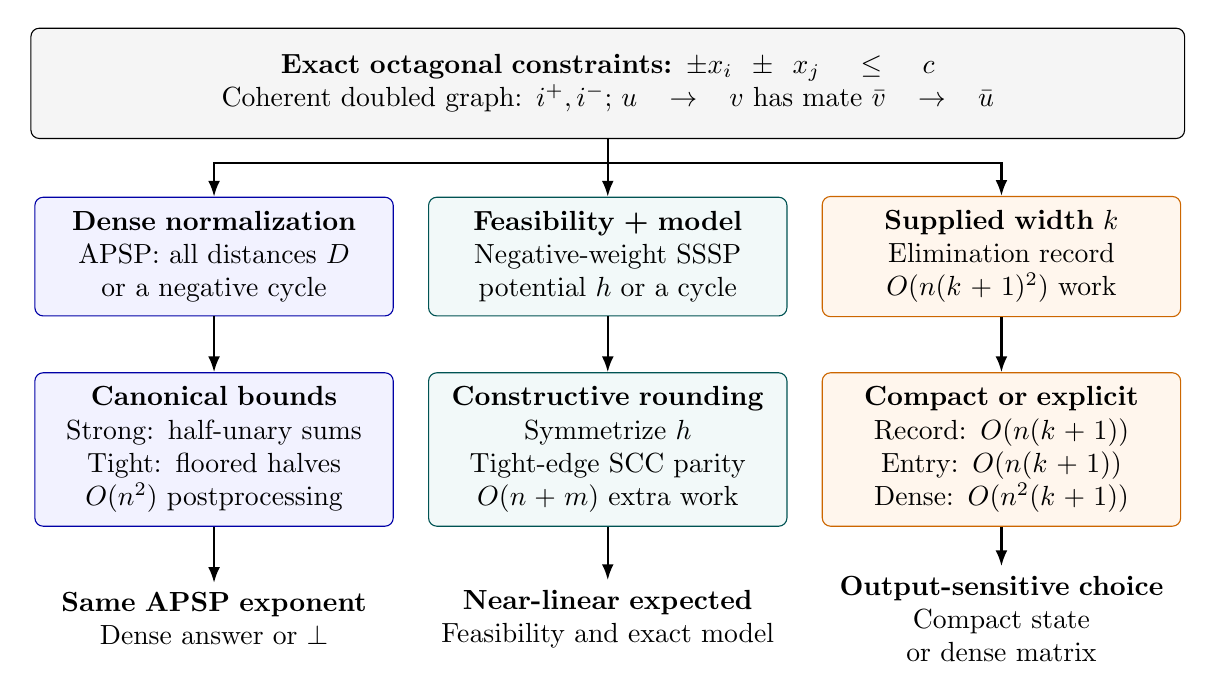
\begin{tikzpicture}[font=\normalsize,
 box/.style={draw,rounded corners=3pt,align=center,minimum height=14mm,inner sep=5pt,text width=42mm},
 arr/.style={-{Latex[length=2mm]},thick},
 dense/.style={box,draw=blue!65!black,fill=blue!5},
 feas/.style={box,draw=teal!65!black,fill=teal!5},
 width/.style={box,draw=orange!80!black,fill=orange!7}]
\node[box,text width=143mm,fill=black!4] (input) at (0,0)
 {\textbf{Exact octagonal constraints: $\pm x_i\pm x_j\leq c$}\\
 Coherent doubled graph: $i^+,i^-$; $u\to v$ has mate $\bar v\to\bar u$};
\node[dense] (a) at (-5,-2.2) {\textbf{Dense normalization}\\APSP: all distances $D$\\or a negative cycle};
\node[feas] (b) at (0,-2.2) {\textbf{Feasibility + model}\\Negative-weight SSSP\\potential $h$ or a cycle};
\node[width] (c) at (5,-2.2) {\textbf{Supplied width $k$}\\Elimination record\\$O(n(k+1)^2)$ work};
\draw[arr] (input.south)--++(0,-.3)-|(a.north);
\draw[arr] (input.south)--(b.north);
\draw[arr] (input.south)--++(0,-.3)-|(c.north);
\node[dense] (d) at (-5,-4.65) {\textbf{Canonical bounds}\\Strong: half-unary sums\\Tight: floored halves\\$O(n^2)$ postprocessing};
\node[feas] (e) at (0,-4.65) {\textbf{Constructive rounding}\\Symmetrize $h$\\Tight-edge SCC parity\\$O(n+m)$ extra work};
\node[width] (f) at (5,-4.65) {\textbf{Compact or explicit}\\Record: $O(n(k+1))$\\Entry: $O(n(k+1))$\\Dense: $O(n^2(k+1))$};
\draw[arr] (a)--(d);\draw[arr] (b)--(e);\draw[arr] (c)--(f);
\node[align=center,text width=45mm] (out1) at (-5,-6.8) {\textbf{Same APSP exponent}\\Dense answer or $\bot$};
\node[align=center,text width=45mm] (out2) at (0,-6.8) {\textbf{Near-linear expected}\\Feasibility and exact model};
\node[align=center,text width=45mm] (out3) at (5,-6.8) {\textbf{Output-sensitive choice}\\Compact state or dense matrix};
\draw[arr] (d)--(out1);\draw[arr] (e)--(out2);\draw[arr] (f)--(out3);
\end{tikzpicture}

\caption{\OctaFine: exact interfaces and where their costs arise. The input has $n$ variables and $m$ constraints; $k$ is a supplied signed-graph elimination width. Solid arrows are algorithmic routes. The left route materializes every pair. On integer inputs, the decision route adds a tight-edge parity/SCC check after a potential is found. The width route separates compact storage from optional dense reconstruction.}
\Description{A coherent doubled graph feeds three separate routes. APSP and a quadratic strengthening pass produce a dense canonical matrix. Negative-weight SSSP and linear SCC rounding produce feasibility and a model. A supplied width order feeds elimination and either an entry oracle or dense reconstruction.}
\label{fig:framework}
\end{figure}

\section{Formal interfaces and inherited normalization}\label{sec:formal}
Let $V=\{1^+,1^-,\ldots,n^+,n^-\}$ with a fixed-point-free involution $u\mapsto\bar u$. A valuation is \emph{antisymmetric} if $y_{\bar u}=-y_u$. We use the orientation convention that an edge $u\to v$ of weight $w_{uv}$ encodes $y_v-y_u\leq w_{uv}$. A DBM has a zero diagonal and entries in $\Z\cup\{+\infty\}$ unless specified otherwise. Multiple edges are replaced by their minimum. A coherent matrix satisfies
\begin{equation}\label{eq:coherent}
 M_{uv}=M_{\bar v\bar u}.
\end{equation}
Every input is made coherent by inserting the mate of each edge. A unary inequality $x_i\leq c$ becomes $i^-\to i^+$ of weight $2c$; $-x_i\leq c$ is analogous. We also allow integral bounds on $2x_i$, which the integer algorithm handles by tightening.

A zone has only differences $x_j-x_i\leq c$. Unary bounds can be represented by a distinguished zero anchor; translating all variables including the anchor and then setting the anchor to zero preserves difference constraints. Adding an anchor increases a supplied decomposition's width by at most one. Our reductions use no anchor or unary bounds. All closure functions return a distinguished $\bot$ on infeasible inputs; on feasible inputs they return the exact matrix of strongest implied signed-difference bounds. Rational closure values may be half-integral. An integer tight matrix has even complementary entries because they encode bounds on $2x_i$.

The following classical normalization theorem supplies the canonical matrices used in our reductions. The rational version follows from the strong-closure results in~\cite{bhz2009}; the integer version is the tight-closure theorem of~\cite{bhz2008}. Their formulas also appear in later treatments~\cite{crk2019,schwarz2023}.

\begin{proposition}[Classical normalization formulas]\label{prop:normal}
Let $D$ be the all-pairs distance matrix of a coherent graph without negative cycles. The rational canonical matrix is
\begin{equation}\label{eq:strong}
 S_{uv}=\min\{D_{uv},(D_{u\bar u}+D_{\bar v v})/2\}.
\end{equation}
For integer weights, put $a_u=\lfloor D_{u\bar u}/2\rfloor$, with $a_u=+\infty$ when this distance is infinite. The system has an integer solution exactly when $a_u+a_{\bar u}\geq0$ for all $u$. If so, its integer canonical matrix is
\begin{equation}\label{eq:tight}
 T_{uv}=\min\{D_{uv},a_u+a_{\bar v}\}.
\end{equation}
\end{proposition}
The fact is invoked with its feasibility and coherence hypotheses. Arithmetic with $+\infty$ uses the usual absorbing conventions. No expression here subtracts infinities. These formulas establish $O(n^2)$ \emph{postprocessing}; computing the prerequisite $D$ remains the expensive part. The integer feasibility criterion is independently proved without APSP in Section~\ref{sec:feasibility}.

\begin{definition}[Subcubic reduction]\label{def:red}
Following Definition 3.1 of~\cite{vvw2018}, $A\leq_3 B$ means that for every $\varepsilon>0$ there exist $\delta>0$, $d>0$, and an oracle algorithm solving $A$, with non-oracle time $O(s^{3-\delta})$ on size-$s$ instances, whose oracle instance sizes $s_i$ satisfy $\sum_i s_i^{3-\varepsilon}\leq d s^{3-\delta}$. Size includes a fixed polynomial in the bit length of weights; equivalently our dimension bounds are accompanied by $\polylog(nW)$ factors. Write $A\equiv_3B$ for reductions in both directions.
\end{definition}
For dimension arguments it suffices to consider $0<\varepsilon\leq1$: a faster oracle can be charged at exponent two if necessary. Our unrestricted closure reductions use a constant number of $O(n)$-dimension calls. The feasible-DAG restriction uses $O(\log n)$ calls. In both cases, weights grow by at most a factor polynomial in $n$. Thus the oracle-budget condition holds with, for example, $\delta=\varepsilon/2$ after absorbing polylogarithmic dimension factors. For arbitrary weight bit lengths, the same statement uses the size measure in Definition~\ref{def:red}, taking its fixed bit-length power large enough for the displayed arithmetic and construction costs.

We use APSP with global negative-cycle reporting: return a negative-cycle flag if any negative cycle exists, and otherwise return all distances. On negative-cycle-free inputs this is ordinary APSP. A min-plus implementation provides this reporting convention by repeated squaring and a negative-diagonal test. The min-plus encoding used for the feasible-oracle restriction is a DAG before coherent duplication.

\section{Proof of closure equivalence}\label{sec:closureproof}
\begin{lemma}[Closure reduces to APSP]\label{lem:upper}
Each closure problem in Theorem~\ref{thm:A} reduces to one APSP instance of $O(n)$ vertices, followed by $O(n^2)$ arithmetic operations.
\end{lemma}
\begin{proof}
For a zone, shortest paths are its closure. A negative cycle is infeasibility; otherwise path inequalities give the canonical difference bounds. For an octagon, construct its coherent graph and run APSP. A negative cycle rules out any signed valuation. If no negative cycle exists, a feasible potential exists, and its antisymmetric average is a rational solution, as also shown in Lemma~\ref{lem:rational}. Apply~\eqref{eq:strong} for rational closure. For integer closure, test the $2n$ complementary-pair conditions of Proposition~\ref{prop:normal}; report $\bot$ on failure and otherwise apply~\eqref{eq:tight}. The graph has $2n$ vertices. Coherent duplication and all formula evaluations use $O(n^2)$ work on a dense input. Finite distances have magnitude at most $(2n-1)W$, since a shortest finite path can be made simple. The output and intermediate arithmetic therefore use $O(\log(nW))$ bits, apart from the single denominator two in strong closure.
\end{proof}

\begin{lemma}[Direct graph embedding]\label{lem:direct}
APSP with global negative-cycle reporting reduces to one unrestricted zone, strong, or tight closure call on $n$ variables, with $O(n^2)$ additional work and unchanged finite weights.
\end{lemma}
\begin{proof}
For every edge $i\to j$ of weight $w_{ij}$ impose $x_j-x_i\leq w_{ij}$. A negative self-loop can be reported immediately; otherwise retain zero diagonal entries. Zone closure is exactly the distance matrix or $\bot$ when there is a negative cycle. For octagons, coherent duplication produces two disjoint signed copies: the input graph on positive vertices and its reversal on negative vertices. A negative cycle exists in the doubled graph exactly when one exists in the input graph, and then the difference system is infeasible. Otherwise every complementary-pair distance is infinite, so both classical strengthening formulas leave the ordinary distances unchanged. Integer potentials exist for integer-weight graphs without negative cycles, hence the tight-closure call introduces no additional infeasibility. Extract the positive block in $O(n^2)$ work. Every graph vertex becomes one program variable, and every input edge contributes at most its coherent mate.
\end{proof}

\begin{lemma}[Feasible product encoding]\label{lem:product}
Given two $r\times r$ matrices $A,B$ with integer entries in $[-W,W]$, their min-plus product reduces to one call to any closure function in Theorem~\ref{thm:A}, on $3r$ variables, with $O(r^2)$ other work. Its graph is feasible and has only difference constraints.
\end{lemma}
\begin{proof}
Use variables $\ell_1,\ldots,\ell_r$, $z_1,\ldots,z_r$, and $q_1,\ldots,q_r$. Insert
\[
 z_j-\ell_i\leq A_{ij},\qquad q_k-z_j\leq B_{jk}.
\]
The constraint graph is the directed three-layer DAG $L\to Z\to Q$. Every $\ell_i$--$q_k$ path has precisely two edges, so its distance is $\min_j(A_{ij}+B_{jk})$. A potential exists for every weighted DAG. With integer weights it can be chosen integral, so this system is feasible over both $\Q$ and $\Z$.

For a zone, read the corresponding entries of its ordinary closure. For an octagon, coherent duplication gives a positive copy of the DAG and a disjoint negative copy with all edges reversed. No vertex can reach its complement. Hence $D_{u\bar u}=+\infty$ for all $u$. The second argument in both~\eqref{eq:strong} and~\eqref{eq:tight} is infinite, and both canonical closures coincide with the ordinary distance matrix. In particular, integer tightening does not alter the desired product entries. Reading the $r^2$ entries completes the reduction.
\end{proof}

\begin{proof}[Proof of Theorem~\ref{thm:A} and Corollary~\ref{cor:2026}]
Lemmas~\ref{lem:upper} and~\ref{lem:direct} prove the constant-call reductions. On polynomial-weight inputs, quadratic construction/extraction and constant dimension blowup preserve every exponent above two. Taking infima proves the asserted equality, including the quadratic endpoint. Closure outputs over rational variables are half-integral; storing each as twice its value preserves the $O(\log(nW))$-bit word size.

For the feasible-DAG promise, Lemma~\ref{lem:product} computes a min-plus product using one feasible closure call. Repeated squaring of a zero-diagonal adjacency matrix computes APSP in $O(\log n)$ such products: a power bound of at least $n$ detects a negative cycle by a negative diagonal; in its absence every finite distance has a simple witness of at most $n-1$ edges. The final power bound is less than $2n$, so finite entries stay within $O(nW)$. If an oracle requires finite matrices, replace infinity within each product by a sentinel larger than $16nW$ and threshold values above $4nW$ back to infinity. Each finite operand has magnitude at most $2nW$; a summand containing the sentinel stays above this threshold. All promise-oracle calls remain feasible DAGs. Logarithmically many calls preserve polynomial exponents.

For the formal subcubic budget, constant-call reductions have total oracle charge $O((cn)^{3-\varepsilon})$; the promised restriction has $O(\log n\,(cn)^{3-\varepsilon})$. Both satisfy Definition~\ref{def:red} with a smaller positive saving, for example $\delta=\varepsilon/2$ for $0<\varepsilon\leq1$, after logarithmic factors are absorbed. The non-oracle work is at most $O(n^2\log n)$.

For Corollary~\ref{cor:2026}, substitute the reported min-plus/APSP running times from~\cite{alman2026,saha2026,majdoddin2026} into these upper reductions. On arbitrary raw inputs, use the min-plus repeated-squaring implementation to include negative-cycle reporting; it incurs only logarithmically many products. Then apply Proposition~\ref{prop:normal}, including the integer consistency test. A factor of $O(\log n)$ is absorbed by $n^{o(1)}$ or $\widetilde O$, as displayed. This proves the transfer for feasible and infeasible inputs with the stated numerical encodings.
\end{proof}

\section{Treewidth, elimination, and explicit output}\label{sec:width}
Let the variable-interaction graph have one vertex per program variable and an undirected edge for every binary input constraint. Unary constraints do not add edges. Replacing every occurrence of a variable in every bag of a width-$t$ tree decomposition by both signed vertices gives bags of size at most $2(t+1)$. Each signed edge is covered, each vertex's bags are connected, and unary complement edges are covered too. The signed graph consequently has width at most $2t+1$. This bound is for the original graph, not its full closure.

We describe the graph algorithm for $N$ vertices and a supplied elimination order with at most $k$ later neighbors in its filled undirected graph. Such an order is obtained from a supplied width-$k$ decomposition by deleting a vertex occurring only in a leaf bag after removing redundant leaf bags; its remaining neighbors lie in that bag. Repeating gives the required ordering. The decomposition's encoding and conversion cost are charged separately if it is not already reduced to an $O(N)$-bag description; its natural size may otherwise exceed the graph size.

\begin{lemma}[Elimination invariant]\label{lem:elim}
Removing vertices in this order, replacing every pair of later neighbors $a,b$ of $v$ by
\begin{equation}\label{eq:elim}
 w_{ab}\leftarrow\min\{w_{ab},w_{av}+w_{vb}\},
\end{equation}
preserves distances among surviving vertices. Store the incident weights of $v$ at its removal. On a negative-cycle-free graph the total work is $O(M+N(k+1)^2)$ and the stored record has $O(N(k+1))$ entries.
\end{lemma}
\begin{proof}
Inductively, each current edge represents a shortest walk between its endpoints whose internal vertices have already been removed. Allowing $v$ as an additional internal vertex either leaves the edge unchanged or concatenates an $a$--$v$ and a $v$--$b$ walk. A shortest walk can be taken to use $v$ at most once because closed walks have nonnegative weight. This gives~\eqref{eq:elim} and the invariant. Each inserted edge has a witness walk in the original graph, so shortcuts cannot introduce a smaller nonexistent distance. Every path through a removed vertex can conversely be replaced by a shortcut. Thus surviving-vertex distances are preserved.

There are at most $k$ later neighbors and at most $(k+1)^2$ pair relaxations per removal. Missing arcs have infinite weight; structural fill connects all undirected neighbor pairs even if a particular directed weight stays infinite. Store both directed incident weights for each later neighbor. The width bound limits this to $O(N(k+1))$ entries. For deterministic constant-time relaxation access, enumerate the $O(N(k+1)^2)$ structural pair tasks in advance, radix-sort their integer endpoint pairs, and assign pointers into the $O(N(k+1))$ distinct filled-edge records. Restore task order by elimination rank before execution. This uses $O(N(k+1)^2)$ temporary storage and time; the final stored record remains $O(N(k+1))$. Input duplicates are coalesced by the same radix-sorting method, with their cost charged in $M$.
\end{proof}

\begin{lemma}[Exact queries and reconstruction]\label{lem:recover}
An elimination record from Lemma~\ref{lem:elim} answers a distance query in $O(N(k+1))$ time. All distances can be reconstructed in $O(N^2(k+1))$ time.
\end{lemma}
\begin{proof}
Keep each stored arc directed upward or downward according to the endpoint ranks. Repeatedly replace a local minimum internal vertex on a path by the shortcut created when it was removed. The stored weight of that shortcut is no greater than the replaced segment. Each replacement shortens the path, so eventually it has no local rank minimum: it first goes upward and then downward, with one highest-rank vertex. Every shortcut has an original-walk witness. Thus the minimum weight over upward-then-downward walks equals the original distance. To find it, initialize the source at zero and all other labels to infinity, relax all upward arcs in increasing order, then relax all downward arcs in decreasing order. These are two DAG passes over $O(N(k+1))$ arcs. They compute the exact distances from the source, including to the queried target.

For the sharper all-pairs accounting use reverse elimination. When $v$ is reinserted, let $S$ be the later vertices and let $K_v\subseteq S$ be its at most $k$ stored neighbors. Distances between vertices of $S$ are already the correct original distances by the elimination invariant. Recover
\[
 d(v,j)=\min_{a\in K_v}\{w_{va}+d(a,j)\},\quad
 d(i,v)=\min_{a\in K_v}\{d(i,a)+w_{av}\}
 \qquad(i,j\in S),
\]
with $d(v,v)=0$. Any original path from or to $v$ has a first or last stored neighbor after lower-ranked internal vertices are shortcut away, proving the $\leq$ directions for these minima. In the other direction, concatenating a stored arc with a correct later-vertex distance gives an original walk, proving the reverse inequalities. A later-vertex distance might itself have a witness through $v$; this is harmless, because concatenated closed subwalks are nonnegative and can be removed. Each reinsertion takes $O(|S|(k+1))$ work. Summing over $v$ gives $O(N^2(k+1))$ and a dense $O(N^2)$ output.
\end{proof}

\begin{proof}[Proof of Theorem~\ref{thm:D}]
Lift the variable decomposition to the signed graph as above, or retain the supplied difference graph for zones. On a feasible input, run Lemma~\ref{lem:elim}. For a strong entry use three distance queries in~\eqref{eq:strong}; for a tight entry use three queries in~\eqref{eq:tight}. The constant factor does not change the query bound. No complementary-pair distances are precomputed for this compact interface. If feasibility is not promised, run Theorem~\ref{thm:B} first; integer infeasibility must not be ignored. For all entries, reconstruct $D$ using Lemma~\ref{lem:recover} and then perform the quadratic pass of Proposition~\ref{prop:normal}. Since $k+1\leq N+1$, the preprocessing term $N(k+1)^2$ is absorbed by $O(N^2(k+1))$. This proves the upper bounds.

For the output obstruction, take a directed path on $n$ vertices with unit weights. Its undirected graph has treewidth one and its closure has a finite entry for each ordered pair in path order. There are $\Theta(n^2)$ such entries, so even reporting only its finite off-diagonal entries requires quadratic output. The graph is a feasible difference system and can also be coherently duplicated without changing this conclusion.

For the combined upper bound, select the smaller of the width-sensitive reconstruction bound and the general-graph bound of Corollary~\ref{cor:2026}. This selection uses the supplied width; no experimental or optimal-width oracle is needed. Reading the input costs $O(m)$ in either case. Finally, supply the three-layer instance in Lemma~\ref{lem:product} with its trivial single-bag decomposition of width $O(n)$. A uniform bound $O(n^2(k+1)^\beta)$ therefore computes the product in $O(n^{2+\beta})$ time. This proves the final algorithm-transfer statement without a complexity hypothesis.
\end{proof}

\paragraph{Relation to decomposition in analyzers.}
Disconnected components allow the graph primitives to run separately. Dense canonical output can introduce cross-component bounds implied by unary constraints; a compact representation can retain those implications until queried. ELINA's online decomposition and split normal forms exploit related structure~\cite{spv2015,gange2021}. Theorem~\ref{thm:D} adds a supplied-width interface that also accommodates connected sparse graphs.

\section{Proof of near-linear feasibility and model construction}\label{sec:feasibility}
We give a self-contained proof of the parity postprocessing, then compose it with the external SSSP theorem. A potential $h$ satisfies $h_v-h_u\leq w_{uv}$ for every edge. An integer potential can be obtained by adding a source with zero-weight edges to every vertex and computing shortest paths, provided there is no negative cycle.

\begin{lemma}[Symmetrization]\label{lem:rational}
A coherent graph has an antisymmetric rational solution if and only if it has no negative cycle. Given an integer feasible potential $h$, $y_u=(h_u-h_{\bar u})/2$ is such a solution and is half-integral.
\end{lemma}
\begin{proof}
A negative cycle contradicts any potential by summing its inequalities. Conversely let $h$ be feasible. For an edge $u\to v$ and its coherent mate $\bar v\to\bar u$, feasibility gives
\[
 h_v-h_u\leq w_{uv},\qquad h_{\bar u}-h_{\bar v}\leq w_{uv}.
\]
Adding and dividing by two proves $y_v-y_u\leq w_{uv}$. The formula makes $y$ antisymmetric. Integer weights yield integer source distances and hence half-integral $y$. Choosing $x_i=y_{i^+}$ gives the required rational model.
\end{proof}

Call $u$ a \emph{half vertex} if $y_u\in\Z+1/2$. Let $H$ contain exactly the edges $u\to v$ between half vertices that are tight at $y$, namely $y_v-y_u=w_{uv}$. Its vertex set can consist of just the half vertices. This graph is coherent: complementing a half vertex preserves its fractional part, and antisymmetry makes the coherent mate of a tight edge tight.

\begin{lemma}[Rounding criterion and construction]\label{lem:rounding}
A coherent integer-weight graph without negative cycles is integer-feasible exactly when no SCC of $H$ contains both $u$ and $\bar u$. When this condition holds, an antisymmetric integer solution is obtained in $O(n+m)$ time from $y$.
\end{lemma}
\begin{proof}
Suppose $u$ and $\bar u$ belong to the same SCC. Tight paths in both directions telescope to weights $y_{\bar u}-y_u$ and $y_u-y_{\bar u}$. Every feasible valuation $z$ must therefore satisfy $z_{\bar u}-z_u=y_{\bar u}-y_u=-2y_u$. For an antisymmetric integer $z$ the left side is even, whereas $2y_u$ is odd. This is impossible.

Conversely assume there is no such SCC. Complementation maps each SCC $C$ to a distinct SCC $\bar C$ and reverses edges in the condensation DAG. Choose a topological order, with ranks increasing along edges between distinct components. Set
\[
 r_u=\begin{cases}
 0,&y_u\in\Z,\\
 +1/2,&y_u\notin\Z\text{ and }\rank(C(u))<\rank(C(\bar u)),\\
 -1/2,&\text{otherwise},
 \end{cases}
 \qquad z_u=y_u+r_u.
\]
Then $z$ is integral and antisymmetric. We check every edge inequality.

If both endpoints are integral, the difference is unchanged. If precisely one is half-integral, its slack $w_{uv}-(y_v-y_u)$ is a nonnegative half-integer, thus at least $1/2$; rounding changes the difference by at most $1/2$. If both are half-integral and the edge is not tight, its slack is a positive integer, thus at least one; rounding changes the difference by at most one.

It remains to check an edge $u\to v$ of $H$, where we need $r_v\leq r_u$. If its endpoints lie in the same component, both have the same rounding choice. Otherwise, a violation would require $r_u=-1/2$ and $r_v=+1/2$. The rank choices and $u\to v$ then imply
\[
 \rank(C(\bar u))<\rank(C(u))<\rank(C(v))<\rank(C(\bar v)).
\]
But the coherent mate gives an edge $C(\bar v)\to C(\bar u)$, forcing the opposite order. This contradiction proves the desired inequality. SCC computation, topological ordering, and the scans all take $O(n+m)$ time and space.
\end{proof}

\begin{lemma}[Relation to the classical potential test]\label{lem:lm}
Let $G_0$ consist of edges with zero reduced cost $w_{uv}+h_u-h_v=0$. The failure condition in Lemma~\ref{lem:rounding} is equivalent to the existence of a vertex $u$ such that $u,\bar u$ lie in one SCC of $G_0$ and $h_u-h_{\bar u}$ is odd. This is the Lahiri--Musuvathi test~\cite{lm2005}.
\end{lemma}
\begin{proof}
The slack of an edge at $y$ is the average of its two nonnegative reduced costs at $h$, for the edge and its coherent mate. Thus every edge tight at $y$ has zero reduced cost at $h$. A conflicting SCC of $H$ is therefore a conflicting SCC of $G_0$, and half-integrality gives odd $h_u-h_{\bar u}$.

Conversely suppose $G_0$ has zero-cost paths from $u$ to $\bar u$ and back, with odd potential difference. Their concatenation is a zero-weight closed walk in the original weights. The coherent reversal of this walk also has total weight zero. All reduced costs at $h$ are nonnegative, so every edge on both walks has zero reduced cost. Every edge of the first walk and its mate are consequently tight at $y$. Moreover along the walk differences of $y$ are integer weights. Since $u$ is a half vertex, all vertices on the walk are half vertices. The two paths belong to $H$ and place $u,\bar u$ in one SCC there.
\end{proof}

\begin{proof}[Proof of Theorem~\ref{thm:B}]
Construct the coherent graph and add a source joined to every signed vertex by a zero-weight edge. It has $O(n+m)$ edges. Apply the Las Vegas negative-weight SSSP theorem of Bernstein--Nanongkai--Wulff-Nilsen~\cite[Theorem 1.1]{bnw2022}. It returns either a negative cycle or exact integer shortest-path distances, in expected $O((n+m)\log^8(n+2)\log W)$ time. The new source makes every negative cycle reachable. Negative-cycle output certifies infeasibility over both number systems. Otherwise the distances give the potential used by Lemma~\ref{lem:rational}. For rational feasibility, return its antisymmetric model. For integer feasibility, apply Lemma~\ref{lem:rounding} and either return its model or its conflicting SCC. Postprocessing costs $O(n+m)$.

If the input variables are integers and an inequality has rational bound $c$, its integral left side is at most $c$ exactly when it is at most $\lfloor c\rfloor$. Unary inequalities are handled before doubling. The reduction therefore applies after reading and rounding the actual rational encodings. On rational variables one may multiply all bounds by a positive common denominator and rescale the model; the resulting logarithmic weight dependence is as specified following the theorem.
\end{proof}

\paragraph{Certificates.}
A returned rational or integer model can be checked by one scan of the constraints. A negative cycle can be checked by summing its weights. In the parity case, extract paths $u\leadsto\bar u\leadsto u$ inside the conflicting SCC. Each path can be chosen simple. The two tight path inequalities force an odd equality on twice an integer, as in Lemma~\ref{lem:rounding}. Together with their original edge identifiers these are an $O(n+m)$-size checkable infeasibility certificate. No all-pairs closure is needed for any of these checks.

\paragraph{What minimum-cost flow supplies.}
The almost-linear minimum-cost-flow result of Chen, Kyng, Liu, Peng, Probst Gutenberg, and Sachdeva~\cite{flow2022} is another route to the graph primitives underlying fast feasibility. One elementary reduction worth distinguishing is negative-cycle detection: assign unit capacities to all graph edges and minimize the cost of a circulation with zero demands. The optimum is negative exactly when a negative cycle exists. In one direction, send one unit along a negative simple cycle. In the other, decompose any negative-cost circulation into nonnegative amounts of directed cycles; one must have negative weight. These instances have integral polynomially bounded capacities and costs when the theorem's hypotheses hold.

The circulation reduction supplies a decision primitive for rational infeasibility. The SSSP interface additionally supplies the potential used for integer parity checking and model construction; its SCC postprocessing remains linear.

\section{Incremental closure and its query model}\label{sec:incremental}
We first verify the upper bound, since the meaning of ``one update'' must not hide an extra closure computation.

\begin{lemma}[Quadratic single-constraint update]\label{lem:incrupper}
Given an ordinary closed distance matrix, inserting one edge can be processed in $O(n^2)$ time. Given a rational strong or integer tight octagon matrix, inserting one octagonal constraint and restoring the same normal form also takes $O(n^2)$ time.
\end{lemma}
\begin{proof}
For one edge $a\to b$ of weight $c$, a negative cycle is created precisely when $D_{ba}+c<0$. If there is no negative cycle, an optimal path can use the inserted edge at most once: remove the segment between two uses, which is a nonnegative closed walk. Hence the new ordinary closure is
\begin{equation}\label{eq:update}
 D'_{ij}=\min\{D_{ij},D_{ia}+c+D_{bj}\}.
\end{equation}
Use the old matrix for all right-hand sides, preserving its row and column or writing into a new matrix. This takes $O(n^2)$ work.

A strong or tight matrix is, in particular, an ordinary closed DBM and is semantically equivalent to its input system. An octagonal constraint inserts at most two coherent edges. Apply the one-edge update twice in sequence, with the intermediate ordinary matrix, checking for negative cycles after each insertion. Coherence is restored after both edges. Replacing the input by its semantically equivalent canonical matrix cannot change the feasible set under further conjunction. Apply Proposition~\ref{prop:normal}, including its integer-consistency check where relevant, to the resulting ordinary closure. This restores the desired canonical form in another $O(n^2)$ pass. This direct argument gives the asymptotic bound; optimized incremental algorithms are developed in~\cite{crk2019}.
\end{proof}

\begin{figure}[H]
\centering
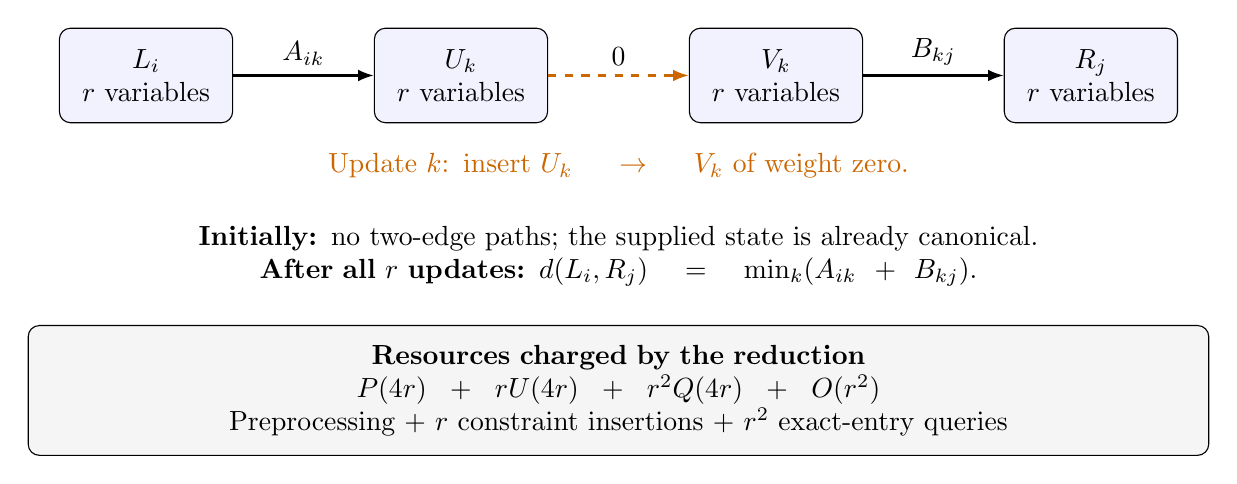
\begin{tikzpicture}[font=\normalsize,
 vertex/.style={draw,rounded corners,minimum width=22mm,minimum height=12mm,fill=blue!5,align=center},
 edge/.style={-{Latex[length=2mm]},thick},
 bridge/.style={edge,dashed,draw=orange!80!black},
 note/.style={align=center,text width=145mm}]
\node[vertex] (l) at (0,0) {$L_i$\\$r$ variables};
\node[vertex] (u) at (4,0) {$U_k$\\$r$ variables};
\node[vertex] (v) at (8,0) {$V_k$\\$r$ variables};
\node[vertex] (r) at (12,0) {$R_j$\\$r$ variables};
\draw[edge] (l)--node[above] {$A_{ik}$}(u);
\draw[bridge] (u)--node[above] {$0$}(v);
\draw[edge] (v)--node[above] {$B_{kj}$}(r);
\node[note,text=orange!80!black] at (6,-1.15) {Update $k$: insert $U_k\to V_k$ of weight zero.};
\node[note] at (6,-2.3) {\textbf{Initially:} no two-edge paths; the supplied state is already canonical.\\
\textbf{After all $r$ updates:} $d(L_i,R_j)=\min_k(A_{ik}+B_{kj})$.};
\node[draw,rounded corners,fill=black!4,note,inner sep=7pt] at (6,-4) {
\textbf{Resources charged by the reduction}\\
$P(4r)+rU(4r)+r^2Q(4r)+O(r^2)$\\
Preprocessing + $r$ constraint insertions + $r^2$ exact-entry queries};
\end{tikzpicture}

\caption{The incremental min-plus encoding. The initial $4r$-variable state contains only the two outer edge families and is already canonical. Inserting bridge $k$ activates product index $k$. Every prefix remains a feasible DAG, with disjoint coherent sign copies. After $r$ insertions, the $r^2$ indicated entry queries recover the product.}
\Description{Four layers L, U, V, and R. Edges L i to U k have weight A i k; edges V k to R j have weight B k j. Bridge U k to V k of weight zero is inserted in update k. Querying the L i to R j distance after all updates returns the minimum over k of A i k plus B k j.}
\label{fig:incremental}
\end{figure}

\begin{proof}[Proof of Theorem~\ref{thm:C}]
For a product of $r\times r$ integer matrices $A,B$, create four layers of variables $L_i,U_j,V_j,R_k$. Initially include only
\[
 U_j-L_i\leq A_{ij},\qquad R_k-V_j\leq B_{jk}.
\]
There is no path of length two in this graph. Its ordinary closure is the adjacency matrix with zero diagonal. On coherent duplication, the signed copies are disjoint and there are no complementary paths. Thus this is also the strong and tight canonical matrix. We can supply the entire initial matrix in $O(r^2)$ work without solving the product.

Insert, for $j=1,\ldots,r$, the single constraints $V_j-U_j\leq0$. In the unsigned graph each gives exactly one bridge; the octagon representation automatically inserts its coherent mate as part of the same constraint update. The graph remains a DAG, the signed copies remain disjoint, and all intermediate systems are feasible over the integers. After all bridges have been inserted, a path from $L_i$ to $R_k$ must take the form
\[
 L_i\longrightarrow U_j\longrightarrow V_j\longrightarrow R_k
\]
for one index $j$. Its weight is $A_{ij}+B_{jk}$, and no other shape of path exists. Strong and tight closure still coincide with ordinary shortest paths. Querying the $r^2$ $L_i$--$R_k$ entries therefore returns $A\otimes B$.

There are $4r$ variables, $r$ constraint insertions, and $r^2$ entry queries. Charging all three resources gives the displayed running time. Substituting their exponents gives a min-plus exponent at most $\max\{2,p,1+u,2+q\}$. Repeated squaring transfers that exponent to APSP, proving~\eqref{eq:tradeoff}. The deterministic statement uses deterministic data structures. For randomized structures the same argument holds with consistent expected-time and error guarantees and the corresponding randomized optimal exponent.
\end{proof}

\begin{proposition}[Explicit-entry writes]\label{prop:writes}
There are feasible difference systems for which one inserted constraint changes $\Theta(n^2)$ canonical entries. An interface requiring each changed entry to be written into its designated storage cell consequently needs $\Omega(n^2)$ work for that update.
\end{proposition}
\begin{proof}
Take $r$ vertices $L_i$, two vertices $a,b$, and $r$ vertices $R_j$. Include zero-weight edges $L_i\to a$ and $b\to R_j$. Initially every $L_i$--$R_j$ distance is infinite. Insert $a\to b$ of weight zero. Every one of these $r^2$ entries becomes zero. The graph is a DAG, so it is feasible. Its coherent duplication has disjoint sign copies, hence gives the same example for rational and integer octagons. Each designated cell must be changed, proving the write lower bound.
\end{proof}
The write bound concerns designated matrix cells. Theorem~\ref{thm:C} additionally covers implicit structures by accounting for the exact-entry queries used to recover the product.

\section{Other abstract operations}\label{sec:operations}
For a nonempty state $P$, let $C(P)_{uv}=\sup_{y\in P}(y_v-y_u)$ over the relevant rational or integer valuations. These are the canonical matrices defined above. Handle $\bot$ separately. Inclusion is semantic inclusion; join is the least octagonal (or zone) upper bound. Widening below is one specified, representation-dependent operation, not a unique semantic operation on all implementations.

\begin{proposition}[Normalized inclusion and join]\label{prop:join}
For feasible canonical matrices $A,B$, inclusion is equivalent to $A_{uv}\leq B_{uv}$ for every entry. The best abstract join is the entrywise maximum $J_{uv}=\max(A_{uv},B_{uv})$, and $J$ is canonical. These operations take $O(n^2)$ time; their dense worst-case complexity is $\Theta(n^2)$.
\end{proposition}
\begin{proof}
If $P\subseteq Q$, taking the supremum of each signed difference gives $C(P)\leq C(Q)$. Conversely every inequality defining $Q$ occurs in its canonical matrix, so $C(P)\leq C(Q)$ implies that every valuation in $P$ satisfies them all. This proves the inclusion test over either number system.

A signed-difference bound valid on both $P$ and $Q$ must be at least the maximum of their two optimal bounds. Their entrywise maximum therefore defines the least representable set containing $P\cup Q$. To verify that its displayed matrix is already canonical, let $R$ be the set it defines. We have $P,Q\subseteq R$, so $C(R)\geq\max(C(P),C(Q))=J$ entrywise, by monotonicity of suprema. Since $R$ is defined by $J$, also $C(R)\leq J$. Thus $C(R)=J$. This proof applies equally to integer canonical bounds, including the even unary entries.

Scanning all entries gives the upper bounds. Outputting a dense join costs $\Omega(n^2)$. For inclusion, consider disjoint variable layers with only constraints $q_j-\ell_i\leq c_{ij}$, where entries $c_{ij}\in\{1,2\}$ are independent and all other nontrivial entries are infinite. These are canonical: no directed path has two edges, and in the doubled graph no complementary path exists. Comparing an all-two first operand against a second operand whose entries are all two, except possibly one hidden one, requires inspecting $\Theta(n^2)$ independent locations in the worst case. This gives the lower bound even for canonical octagons, allowing coherent mates to share storage.
\end{proof}

On raw inputs, one can normalize the antecedent and compare its canonical entries against the explicitly listed consequent inequalities; the consequent need not itself be normalized. This gives an $\Atime+O(n^2)$ dense upper bound for inclusion. Normalizing both operands before computing join gives the same upper bound. This latter bound is APSP-hard when a \emph{canonical} output is required, since joining a raw state with $\bot$ returns its canonical closure. The interface explicitly permits a $\bot$ operand.

Define the classical matrix widening on raw matrices by
\begin{equation}\label{eq:widen}
 (A\mathbin\nabla B)_{uv}=\begin{cases}
 A_{uv},&B_{uv}\leq A_{uv},\\
 +\infty,&\text{otherwise}.
 \end{cases}
\end{equation}
It retains a left-hand constraint if the new state still respects it. Diagonals remain zero, and coherence is preserved if both operands are coherent.

\begin{proposition}[Specified widening interfaces]\label{prop:widen}
Computing~\eqref{eq:widen} with a raw dense output takes $\Theta(n^2)$ time. Computing the separate function $C(A\nabla B)$ on arbitrary raw dense operands is APSP-equivalent. Repeated normalization is a separate termination issue addressed below.
\end{proposition}
\begin{proof}
One entry comparison and assignment per cell computes the raw matrix. It is a sound upper bound for both represented states: it only discards constraints of $A$, and each retained constraint is at least as weak as the corresponding constraint of $B$. Its dense output yields the quadratic lower bound. Across an iteration retaining the previous raw result as the next left operand, a finite entry can only keep its value or become infinite. Each position can be discarded at most once, giving the usual stabilization argument.

For the canonicalized function, first compute the raw result and then close it. Lemma~\ref{lem:upper} gives the APSP upper bound. For the lower bound take $B=A=M$, where $M$ is an arbitrary raw coherent matrix. Then $M\nabla M=M$ syntactically, so the requested output is exactly $C(M)$. Theorem~\ref{thm:A} proves hardness, including on feasible inputs. Normalization can reintroduce finite constraints after they were discarded, so the raw stabilization argument cannot be reused without a separate proof. This distinction is essential in abstract interpretation~\cite{mine2006,bhz2009,gange2021}.
\end{proof}

\section{Computational validation}\label{sec:validation}
We validate the reductions, parity rounding, and graph reconstruction using a dependency-free reference checker, then compare rational strong closure with ELINA's unmodified scalar kernel. OpenAI Codex materially assisted the checker and adapter implementation and the generation of these test protocols; the executed inputs and individual outcomes are archived alongside the source. The potential oracle in the reference checker is Bellman--Ford. This experiment evaluates exact answers, with mathematical running-time guarantees supplied separately by the cited graph algorithms.

\paragraph{Inputs, oracles, and coverage.}
Table~\ref{tab:parameters} records the full generation ranges. Counts distinguish original program variables $n$ from unsigned graph vertices $N$ and product dimension $r$. The number $m$ counts distinct weighted arc records after coherent completion, before taking minima of parallel bounds; for elimination and direct embedding it counts original unsigned graph arcs. Rational-feasible/integer-infeasible cases are identified separately in the per-case records. The principal random seed is $20271031$; the independent ELINA seed is $20271032$.

For integer canonical entries, complete enumeration of $[-3,3]^n$ provides an independent semantic oracle for every output entry. For parity/model checking, compare the classical unsymmetrized SCC criterion, the symmetrized rounding construction, and tight closure, and verify every returned integer model against the original edges. Product reductions are checked against direct min-plus multiplication; incremental cases check every activation prefix. Elimination cases use potential reweightings of nonnegative costs, then compare every reconstructed distance with Floyd--Warshall. An additional direct-embedding suite checks arbitrary signed-weight graphs, including negative-cycle cases, against both octagon normal forms.

\begin{table}[H]
\caption{Executed test coverage and generation parameters. F/I counts are feasible/infeasible cases for the indicated semantics; counts for both rational and integer semantics and observed arc-count distributions are generated from the logs in the artifact. Bounds specify generation ranges, not extrapolated measurements.}
\label{tab:parameters}
\begin{tabularx}{\textwidth}{@{}P{.20\textwidth}Y P{.13\textwidth}P{.18\textwidth}@{}}
\toprule
Family / cases & Generation ranges & Observed $m$ & F/I: $\Q$; $\Z$\\
\midrule
Parity/model / 5000 & $n\in[1,6]$; $[-7,8]$ weights; uniform arc draws, then coherent mates & 0--270 & 1062/3938; 1056/3944\\
Integer enumeration / 600 & $n\in[1,3]$; $[-5,5]$ weights; unary box $[-3,3]^n$ & 2--28 & 223/377; 220/380\\
Static product / 400 & $r\in[1,8]$, $n=3r$; dense $A,B\in[-20,20]^{r\times r}$ & 4--256 & 400/0; 400/0\\
Incremental product / 250 & $r\in[1,6]$, $n=4r$; $A,B\in[-9,9]^{r\times r}$; all prefixes & 6--156 & 250/0; 250/0\\
Elimination / 500 & $N\in[2,23]$; arc probability $0.15$; $w=c+h_v-h_u$, $c\in[0,9]$, $h\in[-20,20]$ & 0--88 & 500/0; 500/0\\
Direct embedding / 500 & $N\in[1,9]$; arc probability $0.3$; integer weights $[-9,9]$ & 0--32 & 273/227; 273/227\\
ELINA kernel / 1000 & $n\in[1,16]$; potential $[-40,40]$, slack $[0,8]$; arc probability $0.2$ & 0--439 & 1000/0; ---\\
\bottomrule
\end{tabularx}

\end{table}

\paragraph{ELINA adapter.}
For revision \texttt{f524156d292a}, compile \path{opt_oct_closure_dense_scalar.c} directly and use the original coherent half-matrix index function in a thin \texttt{ctypes} adapter. Generated rational-feasible states have an antisymmetric integer potential in $[-40,40]$ and nonnegative slack in $\{0,\ldots,8\}$. Their small integral and half-integral answers are exactly representable in binary floating point. The full revision identifier is recorded in the artifact. The $1{,}000$ ELINA cases compare $389{,}512$ entries and remain separate from the reference-check suites. The supplied kernel source, required ELINA headers, source hashes, build command, and adapter make this check reproducible without a live GitHub checkout.

\paragraph{Artifact and recorded outcomes.}
The accompanying \href{run:5_source.zip}{\texttt{5\_source.zip}} contains \path{artifact/validate.py}, \path{artifact/elina_compare.py}, a portable kernel build script, compressed JSONL input fixtures and per-case outcomes, actual stdout logs, and JSON summaries. Paths and file hashes are indexed by \path{artifact/MANIFEST.json}; \path{README.octafine.md} gives the commands. Each JSONL record identifies its suite, parameters, generated input, outcome, and complete checked output with its digest. Seed replay checks the generation stream against the archived inputs. Table~\ref{tab:parameters} is generated from these records, so its totals and feasibility proportions can be recomputed directly. All displayed tests completed without a mismatch. The evidence covers exact kernel and reduction correctness on these finite inputs; the scope paragraph in the introduction specifies the remaining whole-analyzer study.

\section{Related work and implications}\label{sec:related}
\paragraph{Normalization and representations.}
Min\'e's domain~\cite{mine2006}, the strong/tight formulas of Bagnara--Hill--Zaffanella~\cite{bhz2008,bhz2009}, quadratic incremental algorithms~\cite{crk2019}, and the 2-projective account~\cite{schwarz2023} establish the normalization primitives we classify. ELINA's decomposition and kernel optimization~\cite{spv2015} and the split normal forms of~\cite{gange2016,gange2021} exploit state structure and avoid eager dense materialization. Our reductions specify how the cost of exact dense output relates to general graphs.

\paragraph{Feasibility and graph algorithms.}
Lahiri--Musuvathi's potential/SCC criterion~\cite{lm2005} incurs linear work beyond negative-cycle detection. The bit-scaling bound of~\cite{subramani2023} and the SSSP and flow results~\cite{bnw2022,flow2022,bcf2023} supply the quantitative context for Theorem~\ref{thm:B}. The width-sensitive graph primitive comes from classical shortest-path work~\cite{planken2012}. The fine-grained framework is~\cite{vvw2018}; we strengthen its coarse subcubic comparison by retaining linear dimension growth and quadratic overhead.

\paragraph{Consequences and open interfaces.}
The October 2026 results~\cite{alman2026,karingula2026,saha2026,majdoddin2026} make the quantitative version of the reductions central: dense normalization inherits the reported improvements immediately. The next questions concern finer separations. Raw inclusion has an APSP-time upper bound, while its matching exponent remains open here. Boolean-only incremental consistency queries request less information than the exact-entry model of Theorem~\ref{thm:C}. Width-sensitive algorithms leave room to improve the interpolation between compact records and dense output. Measuring these interfaces on program states would connect the classification to analyzer design.

\section*{AI methodology}
OpenAI Codex was used for problem formulation, literature searches, proof development, implementation of the reference checks, and manuscript drafting and typesetting. This materially affected all technical sections and the artifact. The recorded computations are finite validation of the stated constructions; they are not a substitute for the named human authors' responsibility to verify the mathematical arguments, attribution, and originality before submission.

\clearpage
\bibliographystyle{alphaurl}
\bibliography{references}
\end{document}
